\subsection{Понятия структурных схем и структурных преобразований}
Структурная схема~--- это графическое изображение системы в виде блоков с передаточными функциями и связей между ними. На схемах указываеются входныя, промежуточные и выходные переменные.

Структурная схема САУ в простейшем случае строится из элементарных динамических звеньев. Но несколько элементарных звеньев могут быть заменены одним звеном со сложной передаточной функцией. Для этого существуют правила эквивалентного преобразования структурных схем. Рассмотрим возможные способы преобразований для трех элементарных звеньев:
\begin{equation}
    y_1 = W_1 x_1, \quad y_2 = W_2 x_2, \quad y_3 = W_3 x_3.
\end{equation}
\begin{enumerate}
    \item Последовательное соединение:
    \begin{figure}[h!]
        \begin{minipage}[h]{0.5\linewidth}
            \centering{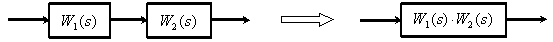
\includegraphics[width=0.5\linewidth]{images/serial.png}}
        \end{minipage}
        \begin{minipage}[h]{0.5\linewidth}
            \begin{equation}
                y = W_1 W_2 W_3 x
            \end{equation}
        \end{minipage}
    \end{figure}
    
    \item Параллельное соединение:
    \begin{figure}[h!]
        \begin{minipage}[h]{0.5\linewidth}
            \centering{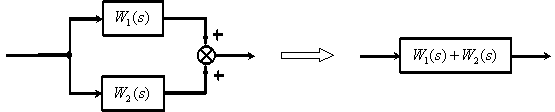
\includegraphics[width=0.5\linewidth]{images/parallel.png}}
        \end{minipage}
        \begin{minipage}[h]{0.5\linewidth}
            \begin{equation}
                y = (W_1 + W_2 + W_3) x
            \end{equation}
    \end{minipage}
    \end{figure}
    
    \item Замкнутая система с ООС (ОС~--- $W_3$):
    \begin{figure}[h!]
        \begin{minipage}[h]{0.5\linewidth}
            \centering{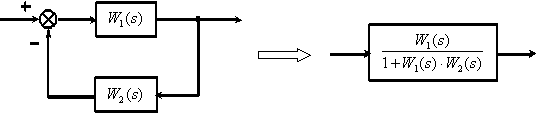
\includegraphics[width=0.5\linewidth]{images/ooc.png}}
        \end{minipage}
        \begin{minipage}[h]{0.5\linewidth}
            \begin{equation}
                y = \cfrac{W_1 W_2}{1 + W_1 W_2 W_3} x
            \end{equation}
        \end{minipage}
    \end{figure}

    \item Замкнутая система с ПОС (ОС~--- $W_3$):
    \begin{figure}[h!]
        \begin{minipage}[h]{0.5\linewidth}
            \centering{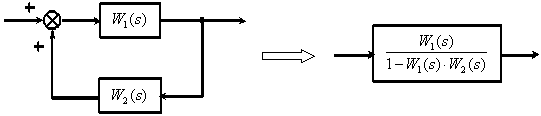
\includegraphics[width=0.5\linewidth]{images/poc.png}}
        \end{minipage}
        \begin{minipage}[h]{0.5\linewidth}
            \begin{equation}
                y = \cfrac{W_1 W_2}{1 - W_1 W_2 W_3} x
            \end{equation}
        \end{minipage}
    \end{figure}
    
    \item Перенос точки ветвления через динамическое звено:
    \begin{figure}[h!]
        \begin{minipage}[h]{0.5\linewidth}
            \centering{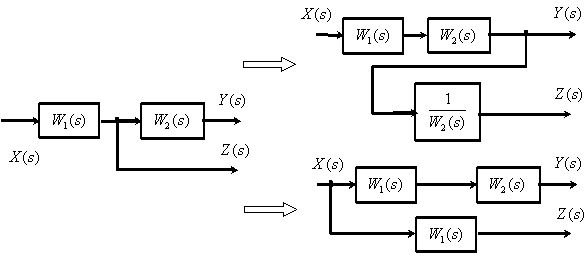
\includegraphics[width=0.5\linewidth]{images/transfer_point.png}}
        \end{minipage}
        \begin{minipage}[h]{0.5\linewidth}
            \begin{gather}
                y = W_1 W_2 x, \\
                z_{fwd} = W_1 W_2 \cfrac{1}{W_2}, \\
                z_{bwd} = W_1
            \end{gather}
        \end{minipage}
    \end{figure}
    
    \item Перенос суммирующего звена через динамическое звено:
    \begin{figure}[h!]
        \begin{minipage}[h]{0.5\linewidth}
            \centering{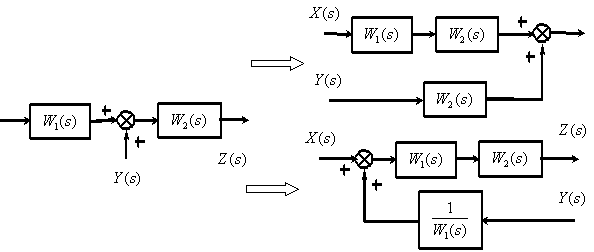
\includegraphics[width=0.5\linewidth]{images/transfer_sum.png}}
        \end{minipage}
        \begin{minipage}[h]{0.5\linewidth}
            \begin{gather}
                z = (W_1+W_2 y) x, \\
                z_{fwd} = W_1 W_2 x + W_2 y, \\
                z_{bwd} = W_1 W_2 (\cfrac{1}{W_2}y + x)
            \end{gather}
        \end{minipage}
    \end{figure}    
\end{enumerate}
    